\section{Discussion}
\label{sec:summary-discussion}

Are there any objects that might not be bow shocks?

Progression in density:
\begin{gather*}
  \text{Increasing density} \longrightarrow \\
  \text{WBS} \to \text{WBS} + \text{IDW} \to \text{WBS} + \text{DDW} \to \text{(RBW)} \to \text{RBS}
\end{gather*}

Chief diagnostic for radiation supported bows (RBW or RBS cases) is
infrared luminosity of bow.  Favored by high densities.

Dust waves favored by high velocities and intermediate densities.


In order to provide an empirical anchor to our theoretical
calculations, we now consider how the parameters of our models might
be determined from observations.  The parameter space diagrams, such
as Figures~\ref{fig:zones-v-n-plane} and
\ref{fig:existence-dust-wave}, are not particularly useful in this
regard, since in many cases the ambient density and relative stellar
velocity are not directly measured.  Instead, we aim to construct
diagnostics based on the most common observations, which are of the
infrared dust emission.

A fundamental parameter is the optical depth, \(\tau\), of the bow shell
to UV radiation, which determines what fraction of the stellar photon
momentum is available to support the shell (see
\S~\ref{sec:three-bow-regimes}).  But the same photons also heat the
dust grains in the bow, which re-radiate that energy predominantly at
mid-infrared wavelengths (roughly \SIrange{10}{100}{\um}) with
luminosity \(L\IR\).  Assuming that Ly\(\alpha\) and mechanical heating of
the dust shell is negligible and that the emitting shell subtends a
solid angle \(\Omega\), as seen from the star, then the optical depth can
be estimated as
\begin{equation}
  \label{eq:tau-empirical}
  \tau = -\ln \left( 1 - \frac{4\pi}{\Omega} \frac{L\IR}{L_*} \right)
  \approx \frac{2 L\IR}{L_*} \ ,
\end{equation}
where the last approximate equality holds if \(\tau \ll 1\) and the
shell emission covers one hemisphere.\footnote{%
  The \(\tau\) of \S~\ref{sec:three-bow-regimes} is not exactly the
  same as the \(\tau\) of equation~\eqref{eq:tau-empirical}, but is
  larger by a factor of
  \(Q_P / Q_{\text{abs}} = 1 + \varpi (1 - g)/(1 - \varpi)\), where
  \(\varpi\) is the grain albedo and \(g\) the scattering asymmetry
  (see App.~\ref{sec:gas-free-bow}).} %

A second important parameter is the thermal plus magnetic pressure in
the shocked shell, which is doubly useful since in a steady state it
is equal to \emph{both} the internal supporting pressure (wind ram
pressure plus absorbed stellar radiation) \emph{and} the external
confining pressure (ram pressure of ambient stream).  The shell
pressure is not given directly by the observations, but can be
determined by the following three steps:
\begin{enumerate}[P1.]
\item \label{P1} The shell mass column (\si{g.cm^{-2}}) can be
  estimated from the optical depth by assuming an effective UV
  opacity: \(\Sigma\shell = \tau / \kappa\)
\item \label{P2} The shell density (\si{g.cm^{-3}}) can be found from
  the mass column if the shell thickness is known:
  \(\rho\shell = \Sigma / h\shell\).  In the absence of other
  information, a fixed fraction of the shell radius can be used.  In
  particular, we normalize by a typical value of
  one~quarter\footnote{%
    This corresponds to a Mach number \(\M_0 = \surd 3\) if the stream
    shock is radiative, or \(\M_0 \gg 1\) if non-radiative (see
    \S~\ref{sec:radi-cool-lengths}).  Further discussion is given in
    Appendix~\ref{app:bow-shock-data}} %
  the star--apex distance: \(h_{1/4} = h\shell / (0.25 R_0)\).
\item \label{P3} Finally, the pressure (\si{dyne.cm^{-2}}) follows by
  assuming values for the sound speed and Alfvén speed:
  \(P\shell = \rho\shell (\sound^2 + \frac12 v\alfven^2) \).
\end{enumerate}
It is natural to normalize this pressure to the stellar radiation
pressure at the shell, so we define a shell momentum efficiency
\newcommand\pc{\ensuremath{_{\text{pc}}}}
\begin{equation}
  \label{eq:eta-shell}
  \eta\shell \equiv \frac{P\shell}{P\rad}
  = \frac{4\pi R_0^2\, (\sound^2 + \frac12 v\alfven^2)\, \tau}{L_*\, \kappa\, h\shell}
  \approx 245 \frac{R\pc \, T_4 \, \tau}{L_4 \, \kappa_{600} \, h_{1/4}} \ , 
\end{equation}
where in the last step we have assumed ionized gas with negligible
magnetic support (\(v\alfven \ll \sound\)) and written the stellar
luminosity and shell parameters in terms of typical values, as in
\S~\ref{sec:depend-stell-type}.  Note that the shell momentum
efficiency is simply the reciprocal of the radiation parameter of
equation~\eqref{eq:Xi-Prad-over-Pgas}:
\(\eta\shell = \Xi\shell^{-1}\), which provides yet a third use for
\(\eta\shell\), since \(\Xi\) is paramount in determining whether the
grains and gas remain well-coupled (see
\S~\ref{sec:exist-cond-separ}).



\begin{table}
  \centering
  \caption[Observational]{Key observational parameters for star/bow systems}
  \label{tab:observations}
  \begin{tabular}{l S S S}
    \toprule
    Star & {\(L_* / \si{L_\odot}\)} & {\(L_{\text{IR}} / \si{L_\odot}\)} & {\(R_0 / \si{pc}\)} \\
    \midrule
    \thD & 2.95e4 & 620 & 0.003 \\
    LP~Ori & 1600 & 240 & 0.01 \\
    \(\sigma\)~Ori & 6e4 & 15 & 0.12 \\[\smallskipamount]
    K18 Sources & \numrange{1.4e4}{8.7e5} & \numrange{8}{2800} & \numrange{0.02}{1.35} \\
    \bottomrule
  \end{tabular}
\end{table}


\begin{figure*}
  \centering
  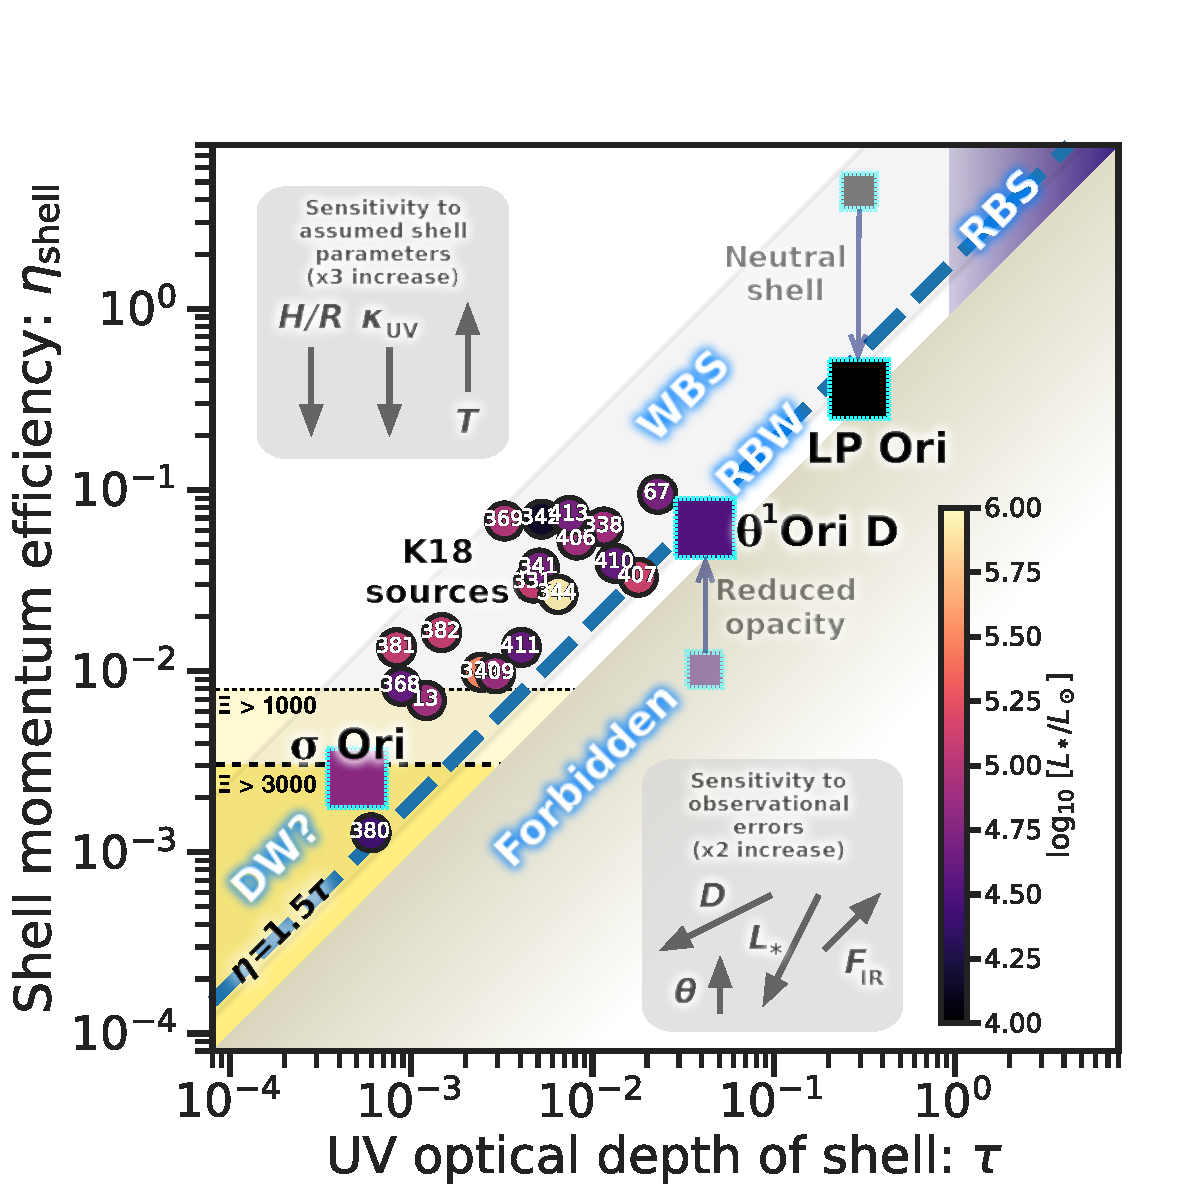
\includegraphics[width=0.8\linewidth]{figs/All-sources-eta-tau}
  \caption[Observational diagnostic diagram]{Observational diagnostic
    diagram for bow shocks.  The shell optical depth \(\tau\) (\(x\)
    axis) and momentum efficiency \(\eta\shell\) (\(y\) axis) can be
    estimated from observations of the bolometric stellar luminosity,
    infrared shell luminosity, and shell radius, as described in the
    text.  Results are shown for the 20 sources (circle symbols) from
    \citet{Kobulnicky:2018a} plus three further sources (square
    symbols), where we have obtained the measurements ourselves (see
    Tab.~\ref{tab:observations}).  The color of each symbol indicates
    the stellar luminosity (dark to light) as indicated by the scale
    bar. The shell pressure is determined assuming a gas temperature
    \(T = \SI{e4}{K}\), an absorption opacity
    \(\kappa = \SI{600}{cm^2.g^{-1}}\), and a thickness-to-radius ratio
    \(H/R = 0.25\).  The sensitivity of the results to a
    factor-of-three change in each parameter is shown in the upper
    inset box.  Exceptions are the two Orion Nebula sources, \thD{}
    and LP~Ori, where the small dim squares show the results of
    assuming the standard shell parameters, while the large squares
    show the results of modifications according to the peculiar
    circumstances of each object, as described in the text.  The lower
    inset box shows the sensitivity of the results to a factor-of-two
    uncertainty in each observed quantity: distance to source \(D\);
    stellar luminosity \(L_*\), shell infrared flux \(F\IR\); shell
    angular size \(\theta\).  Lines and shading indicate different
    theoretical bow regimes (see \S\S~\ref{sec:strong-gas-grain} and
    \ref{sec:imperf-coupl-betw}).  The dashed blue diagonal line
    corresponds to radiation-supported bows, while the upper left
    region corresponds to wind-supported bows.  The upper right corner
    (purple) corresponds to optically thick bow shocks, while the
    lower left corner (yellow) is the region where grain--gas
    separation \textit{may} occur, leading to a potential dust wave.
    However, the existence of a dust wave in this region is not
    automatic, since it only includes one of the four necessary
    conditions (\S~\ref{sec:exist-cond-separ} and
    \S~\ref{sec:grain-traj-with}). The lower-right region is strictly
    forbidden, except in case of violation of the assumption that dust
    heating be dominated by stellar radiation. }
  \label{fig:All-sources-eta-tau}
\end{figure*}


In Figure~\ref{fig:All-sources-eta-tau} we show the resultant
diagnostic diagram: \(\eta\shell\) versus \(\tau\).  The horizontal
axis shows the fraction of the stellar radiative \emph{energy} that is
reprocessed by the bow shell, while the vertical axis shows the
fraction of stellar radiative \emph{momentum} that is imparted to the
shell, either directly by absorption, or indirectly by the stellar
wind (which is itself radiatively driven).  Radiatively supported bows
(DW, RBW, or RBS, or cases) should lie on the diagonal line
\(\eta\shell = ( Q_P / Q_{\text{abs}}) \tau \approx 1.25 \tau\), where
we have used the ratio of grain radiation pressure efficiency to
absorption efficiency found in the FUV band for the dust mixture shown
in Figure~\ref{fig:cloudy-ism-dust-opacity}.  Wind-supported bows
should lie above this line and no bows should lie below the
\(\eta = \tau\) line, since \(Q_P\) cannot be smaller than
\(Q_{\text{abs}}\).

We have calculated \(\eta\shell\) and \(\tau\) using the
above-described methods for the 20 mid-infrared sources studied by
\citet{Kobulnicky:2018a} (K18) and plotted them on our diagnostic
diagram.  Details of our treatment of this observational material are
provided in Appendix~\ref{app:bow-shock-data}.  In order to expand the
range of physical conditions, we have included three additional
sources (data in Table~\ref{tab:observations}): bows around \thD{}
\citep{Smith:2005a} and LP~Ori \citep{ODell:2001c} in the Orion
Nebula, which show larger optical depths, plus the inner bow around
\(\sigma\)~Ori, which illuminates the Horsehead Nebula and has
previously been claimed to be a dust wave \citep{Ochsendorf:2014b,
  Ochsendorf:2015a}.  Details of the observations of these additional
sources will be published elsewhere.

Rather than clutter the diagram with error bars, we instead show the
sensitivity to observational errors in the lower-right box, where each
arrow corresponds to a factor of two increase (0.3~dex) in an
observational quantity: distance, \(D\); stellar luminosity, \(L_*\);
total infrared flux, \(F_{\text{IR}}\); and bow angular apex distance,
\(\theta\).  In \S~\ref{app:bow-shock-data} we estimate the
uncertainty in each observational quantity, which we then combine to
find the \(\pm 1~\sigma\) error ellipse shown in blue in the figure.
It can be seen that observational uncertainties in \(\tau\) and
\(\eta\) are highly correlated: the dispersion is \SI{0.7}{dex} in the
product \(\eta\tau\) but only \SI{0.16}{dex} in the ratio
\(\eta/\tau\), with stellar luminosity errors dominating in both
cases.  Observational uncertainties are therefore relatively
unimportant in determining whether a given source is wind-driven or
radiation-driven.


Mass loss rates - starting from \citet{Kobulnicky:2010a}

\begin{figure*}
  \centering
  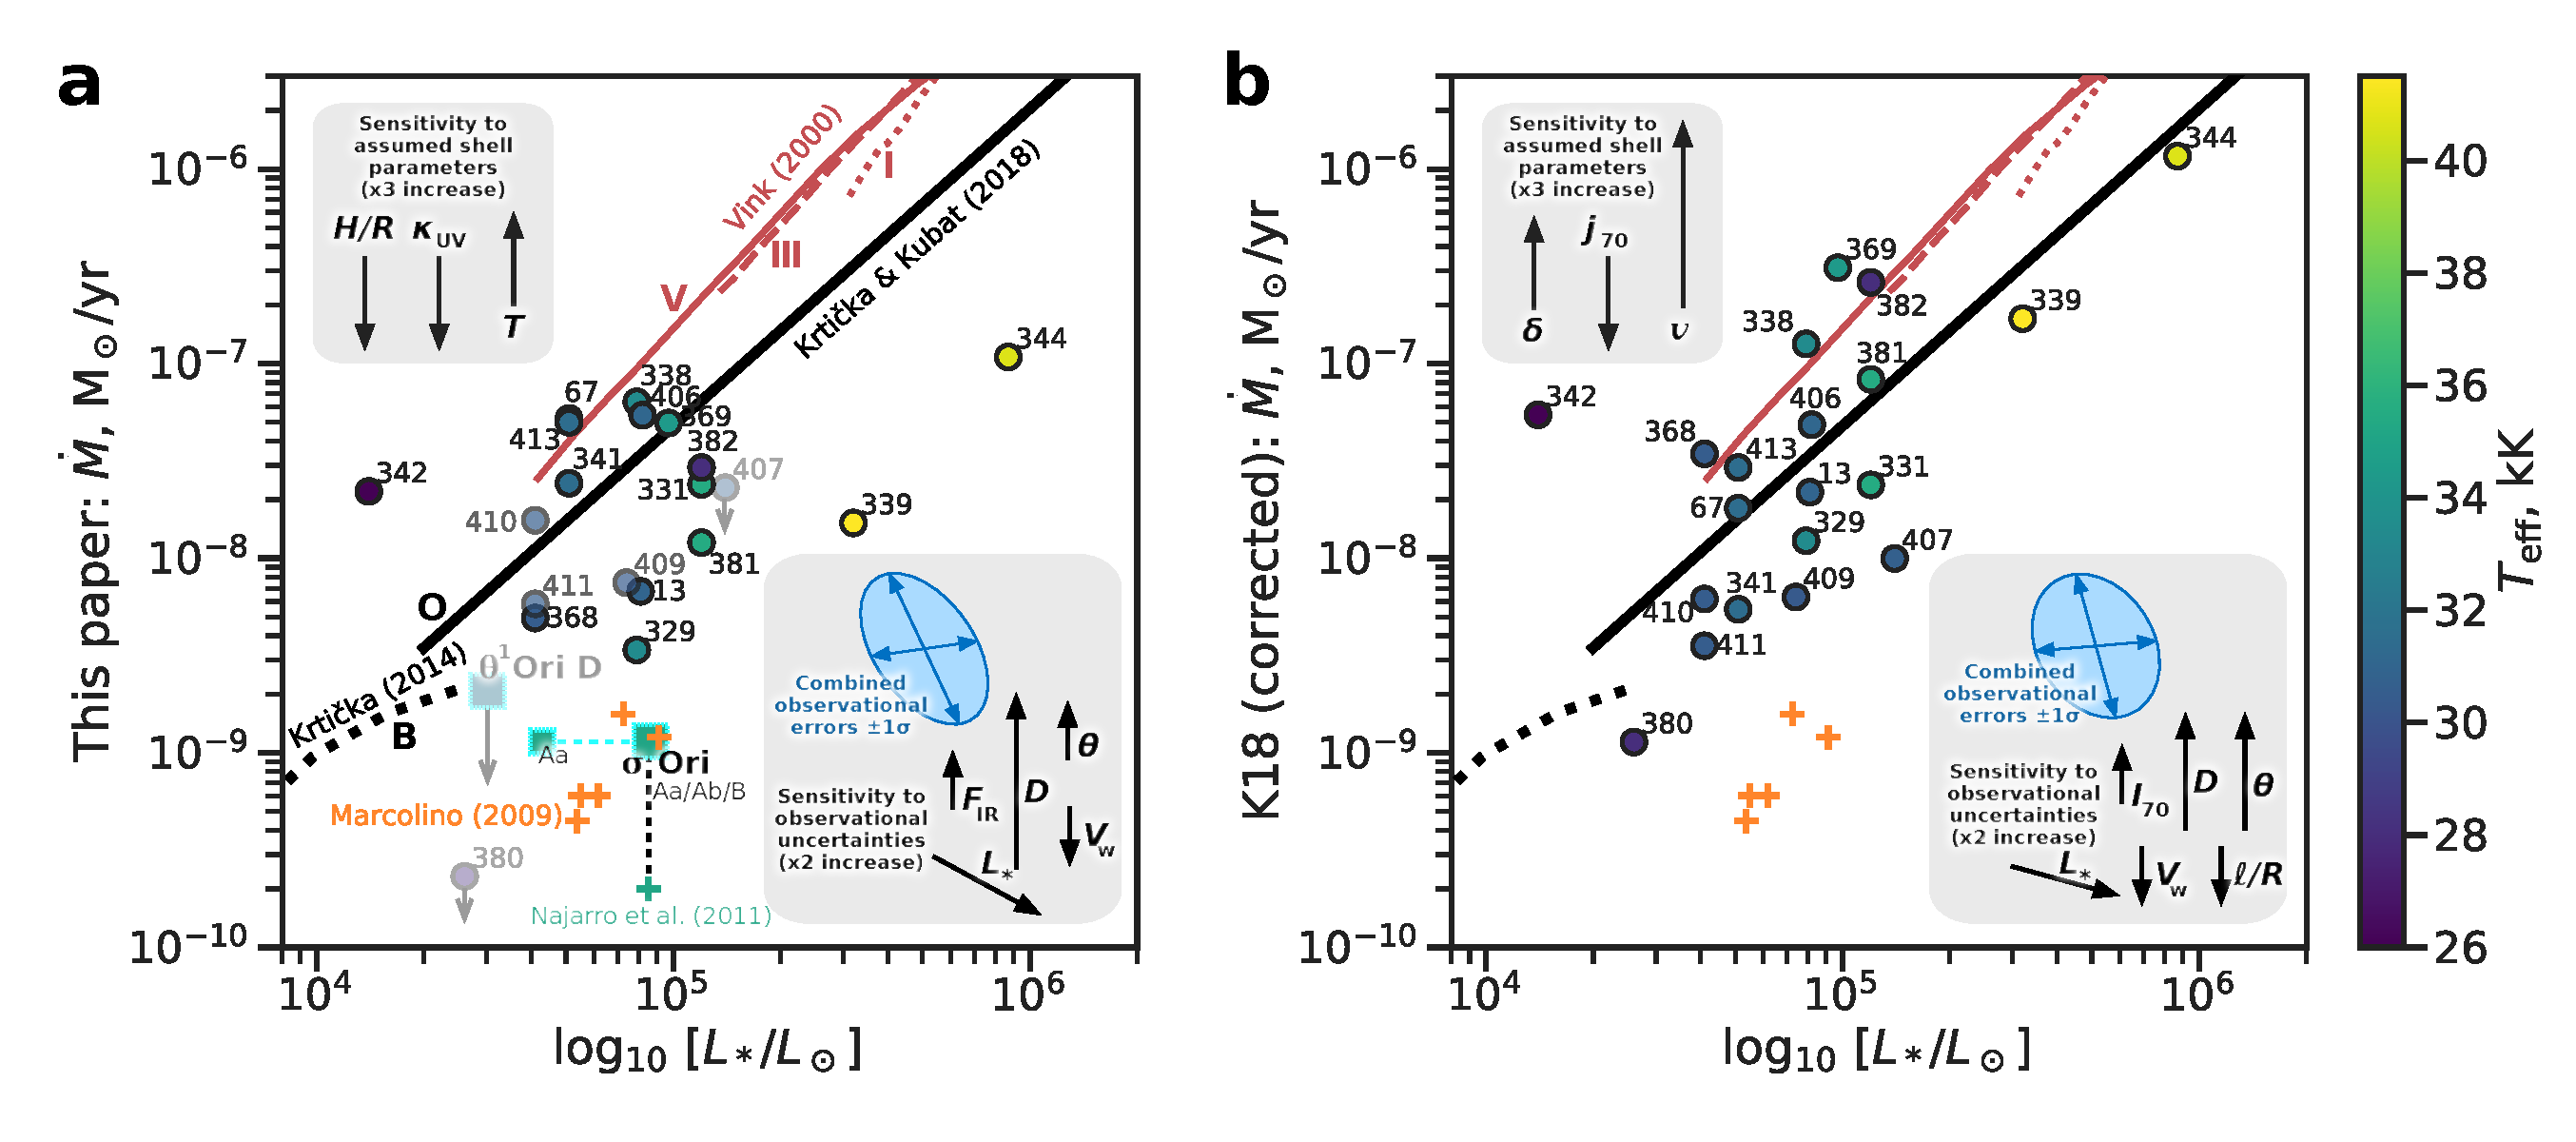
\includegraphics[width=\linewidth]{figs/Mdot-vs-lum-combo-edited}
  \caption{Wind mass-loss rates as a function of stellar luminosity,
    derived from (a)~our trapped energy/momentum method and (b)~the
    grain emissivity method of \citet{Kobulnicky:2018a}, with
    corrections as described in our Appendix~\ref{app:bow-shock-data}.
    Circle symbols show the sources from K18, colored according to the
    stellar effective temperature (see key at far right). In panel a,
    squares show two of our additional sources
    (Tab.~\ref{tab:observations}). Upper limits to the mass loss are
    given for sources that lie close to the radiation-supported line
    in Fig.~\ref{fig:All-sources-eta-tau}, represented by faint
    symbols and downward-pointing arrows.  Sources that lie less than
    a factor of three above the line have enhanced downward
    uncertainties and are also shown by slightly fainter symbols.  For
    \(\sigma\)~Ori, the large symbol corresponds to the sum of the
    luminosities of the triple OB system Aa, Ab, and B
    \citep{Simon-Diaz:2015a}, while the small symbol corresponds to
    the luminosity of only the most massive component Aa.  Lines show
    the predictions of stellar wind models: red lines are the commonly
    used recipes from \citet{Vink:2000a} for dwarfs (solid), giants
    (dashed), and supergiants (dotted), while black lines show
    eq.~(11) of \citet{Krticka:2017a} for O~stars (solid) and models
    of \citet{Krticka:2014a} for B stars.  Orange plus symbols show
    mass-loss measurements from NUV lines for weak-wind O~dwarfs
    \citep{Marcolino:2009a}, while the green plus symbol shows the
    measurement from infrared H recombination lines for \(\sigma\)~Ori
    \citep{Najarro:2011a}.  Boxes show the sensitivity of the results
    to observational uncertainties (lower right) and assumed shell
    parameters (upper left).}
  \label{fig:mass-loss-vs-luminosity}
\end{figure*}



Different scenarios for producing velocities: dynamic ejection from
young clusters \citep{Hoogerwerf:2001a, Oh:2016c} produce high
velocities, dissolution of binary systems following core-collapse SN
\citep{Renzo:2018a} tend to produce lower velocities for the unbound
MS companion (walkaways, slower than 30 km/s).  Also, champagne flows
have low velocities.

How different regions of the \(\Pi\)--\(\Lambda\) plane are populated.
Bottom-right quadrant hard to get to (except for standing wave
oscillations), but may be due to finite shell thickness, which (for
low Mach number) will be more apparent in the wings, which might
decrease \(\Lambda\) more than \(\Pi\).  Fact that thin-shell solutions should
trace the contact discontinuity, but in some cases it may be only the
inner or the outer shell that is visible.

Justification for standing waves: Fig.~3 of \citet{Meyer:2016a} shows
a time sequence of thin-shell instability, which looks a bit like a
standing wave. But much larger amplitude than we are considering.

Deviations from axisymmetry as an alternative to oscillations. 


\subsection{The case of inside-out bows}
\label{sec:case-inside-out}

So far, we have considered the case where the inner source dominates
the radiation, while dust is present only in the outer stream, which
applies to hot stars interacting with the ISM.  However, in the case
of cool stars, the inner wind will also be dusty.  Examples are the
red supergiant (RSG) phase of high-mass evolution, or the asymptotic
giant branch (AGB) stage of low/intermediate-mass evolution.  In both
these cases, it is still the inner source that provides the radiation
field.  However, not all winds are radiatively driven and in those
cases it is conceivable that it is the outer source that dominates the
radiation field.  An example is the case of photoevaporating
protoplanetary disks (proplyds) in the Orion Nebula and other \hii{}
regions \citep{ODell:1994a}.  In the proplyds, the inner wind is a
thermally driven photoevaporation flow \citep{Henney:1998b, Henney:1999a},
while the outer stream is the stellar wind from an O~star
\citep{Garcia-Arredondo:2001a}.


\section{Summary and conclusions}
\label{sec:conclusions}



%%% Local Variables:
%%% mode: latex
%%% TeX-master: "dusty-bow-wave"
%%% End:
